\documentclass{../zkdl-presentation-template}

\title[Криптографія]{\textbf{Практичне №2.Шифри перестановки}}

\date{9.09.2025}


\begin{document}
    \frame{
        \titlepage
    }
  
    \begin{frame}{Plan}
        \tableofcontents
    \end{frame}

\section{Шифри перестановки} % Note all sections and subsections are automatically placed in your table of contents

%------------------------------------------------
\begin{frame}
    \frametitle{Шифр частоколу}
    \begin{block}{}
        Схема шифрування, де ключем виступає параметр $h$ і визначає висоту тексту. Нижче наведено приклад шифрування повідомлення з допомогою ключа $h=3:$
    \end{block}
    \begin{figure}[h!]
                \centering
                % \caption{Hawkins et al, 2015}
                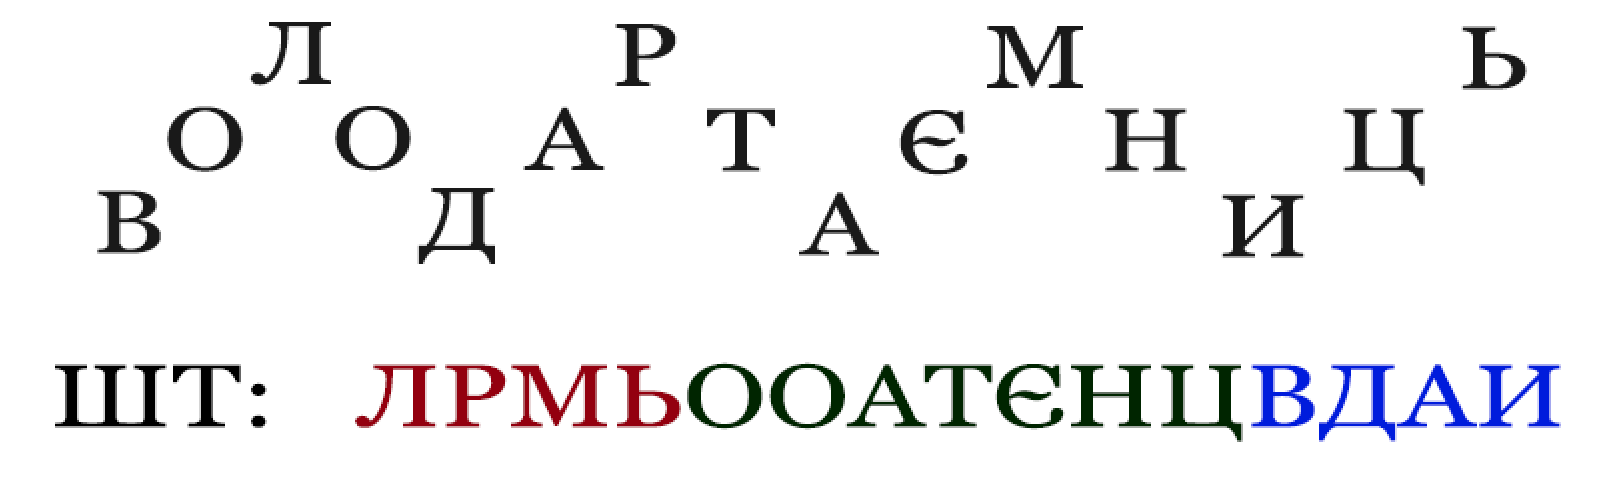
\includegraphics[angle=0, width=10.5cm]{2-crypto-sym/images/ciphkol.png}
                \label{Figure 2}
    \end{figure}

    %\begin{center}
    %    {\Huge\calligra Enjoy!}
    %\end{center}
\end{frame}

%------------------------------------------------
\begin{frame}
    \frametitle{Задачі}
        \begin{block}{}
        \begin{enumerate}
            \item Текст довжиною $9$ літер шифрується шифром частоколу з ключем $3$. Шифрований текст знову шифрується тим самим шифром і т.д. Через скільки кроків буде отримано відкритий текст?
            
            \centering
            
\includegraphics[width=0.95\linewidth]{2-crypto-sym/images/cells.png}

        \end{enumerate}
    	\end{block}
    
\end{frame}
%------------------------------------------------
\begin{frame}
    \frametitle{Задачі}
        \begin{block}{}
        \begin{enumerate}
            \item[2.]	Відкритий текст 
            \vspace{-3mm}
            \begin{align*}
                \texttt{ЯБЛУКОЧЕРВОНЕКИСЛЕ}
            \end{align*}
            
            \vspace{-3mm}
            шифрують шифром блокової перестановки і отримують шифрований текст 
            \vspace{-3mm}
            \begin{align*}
                \texttt{ЧЛЕРЯОУБКСНЛЕВИЕОК}
            \end{align*}

            \vspace{-3mm}
            Цей результат шифрування знову шифрується тим самим шифром перестановки і т. д. Яка довжина блоку використаного шифру? Після якого циклу шифрування знову з’явиться відкритий текст?
        \end{enumerate}
                    \centering
            
\includegraphics[width=0.95\linewidth]{2-crypto-sym/images/cells_small.png}

    	\end{block}
    
\end{frame}
%------------------------------------------------
\begin{frame}
    \frametitle{Задачі}
        \begin{block}{}
        \begin{enumerate}
            \item[3.]	\begin{enumerate}
                \item[a)] Яку потужність ключового простору має шифр табличної перестановки із довжиною блоку п.
                
                \item[b)] Оцініть потужність ключового простору шифру табличної перестановки із довжиною блоку $n$, якщо відомо, що при шифруванні жодна буква не залишається на своєму місці.
            \end{enumerate}
        \end{enumerate}
        
                    \centering
            
\includegraphics[width=0.90\linewidth]{2-crypto-sym/images/cells.png}

    	\end{block}
    
\end{frame}
%------------------------------------------------
\begin{frame}
    \frametitle{Шифр Кардано}
        \begin{block}{Визначення}
        Грати Кардано – це шифр перестановки, секретним ключем якого є сітка (таблиця) розміром $2n \times 2n$ , в якій вирізується $n^2$ віконець (клітинок).
    	\end{block}
        \begin{columns}[c] % [c] вирівнювання по центру вертикалі
        \column{0.5\textwidth}
        \begin{figure}
            \centering
            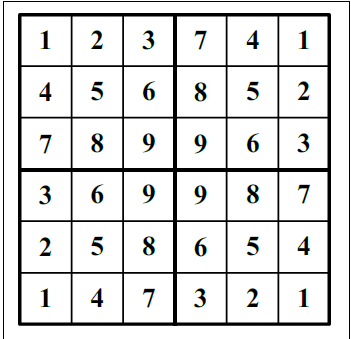
\includegraphics[width=0.75\linewidth]{2-crypto-sym/images/kardano1.png}
            \label{fig:placeholder}
        \end{figure}

        \column{0.5\textwidth}
        \begin{figure}
            \centering
            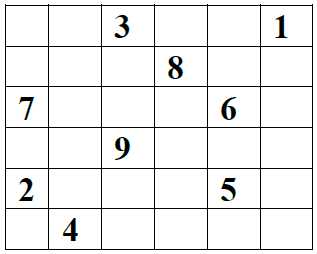
\includegraphics[width=0.75\linewidth]{2-crypto-sym/images/kardano2.png}
            \label{fig:placeholder}
        \end{figure}
    \end{columns}
    
\end{frame}
%------------------------------------------------
\begin{frame}
    \frametitle{Задачі}
        \begin{block}{}
        \begin{enumerate}
            \item[4a] Розшифруйте криптограму задану ключем сітки:
        \end{enumerate}
        
                    \centering
            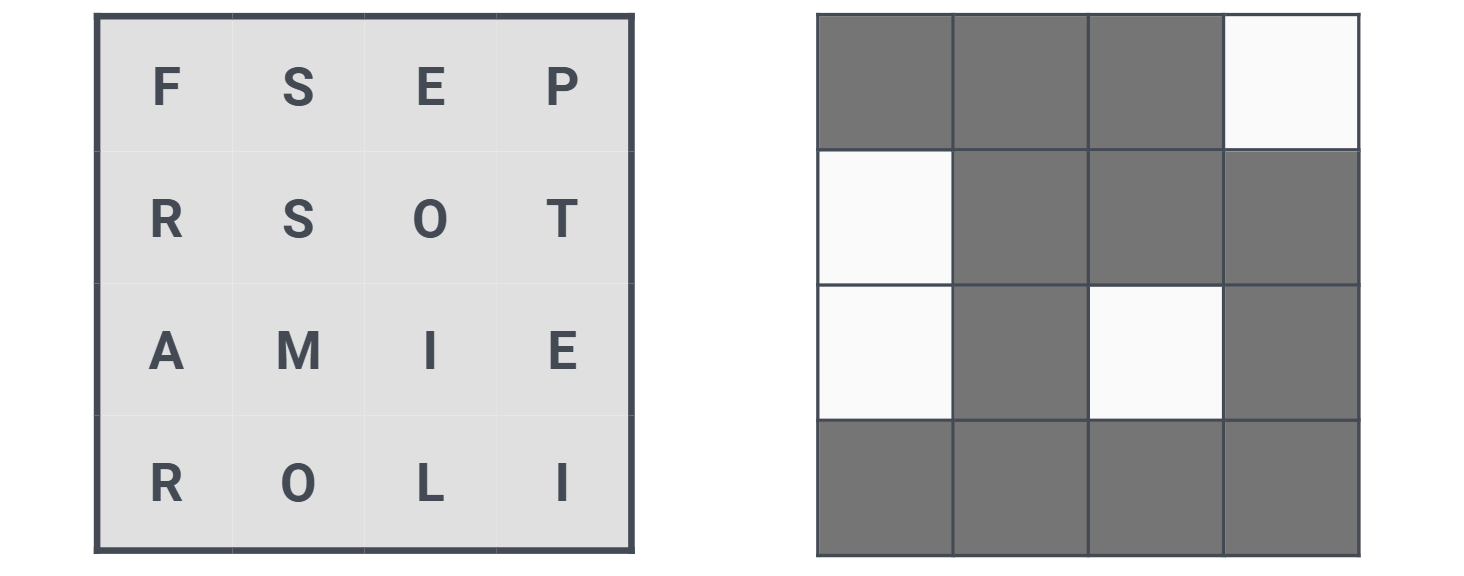
\includegraphics[width=0.75\linewidth]{2-crypto-sym/images/ciphcardano.png}

                    \centering
            
\includegraphics[width=0.95\linewidth]{2-crypto-sym/images/cells_small.png}
    	\end{block}
    
\end{frame}
%------------------------------------------------
\begin{frame}
    \frametitle{Задачі}
        \begin{block}{}
        \begin{enumerate}
            \item[4b] Яку потужність має ключовий простір шифру Кардано із решіткою розміру $2n\times 2n$?
            \item[4c] запропонуйте варіант шифру Кардано із решіткою розміру $(2n+1)\times(2n+1)$. Оцініть потужність ключового простору;
            \item[4d] запропонуйте варіант шифру Кардано із решіткою розміру $(2n)\times(2m)$. Оцініть потужність ключового простору
        \end{enumerate}
                    \centering
            
\includegraphics[width=0.95\linewidth]{2-crypto-sym/images/cells_small.png}    
            
    	\end{block}
    
\end{frame}
%------------------------------------------------
\begin{frame}
    \frametitle{Задачі}
        \begin{block}{}
        \begin{enumerate}
            \item[5] Криптоаналітик перехопив повідомлення, що було зашифроване шифром Кардано, із решіткою розміру $2n\times2n$ . В повідомленні використано $r$ символів <<$*$>> для доповнення відкритого тексту до довжини $4n^2$. Оцініть складність перебору ключового простору, якщо a) $0<r\leq n^2$ ; b) $n<r\leq 2n^2$.
        \end{enumerate}
                    \centering
            
\includegraphics[width=0.95\linewidth]{2-crypto-sym/images/cells_small.png}    
            
    	\end{block}
    
\end{frame}
%------------------------------------------------
\begin{frame}
    \frametitle{Інволютивність шифра}
        \begin{block}{Визначення}
        (Повтор.) Буква $x$ алфавіту $X$ називається нерухомою точкою шифру $E$ з ключем $k$, якщо
        \begin{align*}
            E_K(x)=x
        \end{align*}
        Алгоритм шифрування $E$ називають \textbf{інволютивним}, якщо повторне шифрування призводить до розшифрування:
        \begin{align*}
            \forall x\in X,\forall K: E_K(E_K(x))=x
        \end{align*}
    	\end{block}
        \begin{alertblock}{Задача}
            Нехай шифр заміни інволютивний та не має нерухомих точок. Скільки таких шифрів можна побудувати на алфавіті з $n^2$ символів?
        \end{alertblock}
    
\end{frame}
%------------------------------------------------
\begin{frame}
    \frametitle{Задачі}
        \begin{alertblock}{Задача}
            Шифр Бофора -- модифікація шифру Віженера, де шифрування відбувається за правилом:
            \begin{align*}
                c_i=-m_i+k_i \texttt{ mod n}.
            \end{align*}
            Доведіть, що шифр Бофора інволютивний.
            
                    \centering
            
\includegraphics[width=0.95\linewidth]{2-crypto-sym/images/cells_small.png}              
        \end{alertblock}
    
\end{frame}
%------------------------------------------------
\begin{frame}
    \frametitle{Групова властивість шифру}
\begin{block}{}
    Шифр вважається з груповою властивістю, якщо виконується вимога: $(\forall k_1,k_2\in K)(\exists k_3\in K)(\forall x\in X): E_{K1}(E_{K_2}(x))=E_{K_3}(x)$
\end{block}
\begin{alertblock}{Задачі}
    Чи мають групову властивість шифри:
    \begin{enumerate}
        \item Цезаря
        \item Віженера однакового періоду; різного
        \item Загальної перестановки однак. довжини блоку; різних довжин.
    \end{enumerate}

                    \centering
            
\includegraphics[width=0.95\linewidth]{2-crypto-sym/images/cells_small.png}  
\end{alertblock}
    
\end{frame}
%------------------------------------------------
\section{Ентропія}
\begin{frame}
    \frametitle{Визначення ентропії}
\begin{block}{}
    Ентропія розподілу ймовірностей $p$:

    \vspace{-9mm}
    \begin{align*}
        p=(p(0),p(1),..,p(n-1)),p(i)\geq 0,i=\overline{1,n},\sum_{i=0}^{n-1}p(i)=1
    \end{align*}

    \vspace{-3mm}
    є числом, яке визначається наступним чином:

    \vspace{-7mm}
    \begin{align*}
        H(p)=-\sum_{i=0}^{n-1}p(i)\cdot\texttt{log}p(i)
    \end{align*}
\end{block}
\begin{alertblock}{}
    Розглянемо ансамблі $\langle X,P\rangle$ та $\langle Y,Q\rangle$, де $X=\{x_1,x_2\}$, $Y=\{y_1,y_2,y_3\}$. Який ансамбль має більшу ентропію:
    \begin{enumerate}
        \item $p_1=p_2$, $q_1=q_2=q_3$;
    \end{enumerate}

                    \centering
            
\includegraphics[width=0.95\linewidth]{2-crypto-sym/images/cells_small.png}  
\end{alertblock}
\end{frame}
%------------------------------------------------
\begin{frame}
    \frametitle{Визначення ентропії}
\begin{block}{}
    Ентропія розподілу ймовірностей $p$:

    \vspace{-9mm}
    \begin{align*}
        p=(p(0),p(1),..,p(n-1)),p(i)\geq 0,i=\overline{1,n},\sum_{i=0}^{n-1}p(i)=1
    \end{align*}

    \vspace{-3mm}
    є числом, яке визначається наступним чином:

    \vspace{-7mm}
    \begin{align*}
        H(p)=-\sum_{i=0}^{n-1}p(i)\cdot\texttt{log}p(i)
    \end{align*}
\end{block}
\begin{alertblock}{}
    Розглянемо ансамблі $\langle X,P\rangle$ та $\langle Y,Q\rangle$, де $X=\{x_1,x_2\}$, $Y=\{y_1,y_2,y_3\}$. Який ансамбль має більшу ентропію:
    \begin{enumerate}
        \item $p_1=q_1$, $p_2=q_2+q_3$.
    \end{enumerate}

                    \centering
            
\includegraphics[width=0.95\linewidth]{2-crypto-sym/images/cells_small.png}  
\end{alertblock}
\end{frame}
%------------------------------------------------

    \begin{frame}[plain, standout]
    \begin{figure}
        \centering
        
\includegraphics[width=0.9\linewidth]{Cryptocats.jpg}
        \label{fig:placeholder}
    \end{figure}
    \centering
    \LARGE
    \textbf{Питання?} \\

    \vspace{0.2cm} \Huge \ding{170} \large \\

  \end{frame}
\end{document}